% Chapter 3

\chapter{Development of Artefact and Article} % Main chapter title

\label{Chapter3} % For referencing the chapter elsewhere, use \ref{Chapter3} 

This chapter describes the artefact that was developed in a group effort as well as the process followed for the writing of the academic article.

\section{Description of Artefact and Article}
This research project was split into two main aspects: 
\begin{enumerate}
\item An individual research study into a chosen topic \textit{(this being the qualities needed for a computer game to be used in education)}
\item A group effort to develop a digital computer game.
\end{enumerate}

\noindent For the first aspect of this project, the resulting outcome was an academic article titled, \textit{"Linking Gamification, Ludology and Pedagogy: How to Use Serious Games for Various Knowledge Domains"}. As stipulated in the title, the fields of gamification, ludology and pedagogy were the focus of this research aspect of the project. In this article, the question posed by this project is again reiterated and sequentially answered. The article is attached to this document under Appendix  \ref{AppendixC}. 
\\\\
The artefact accompanying this research project is a digital computer came which was developed as part of a group effort as mentioned previously. While this artefact is separate from the individual research studies conducted by its' group members, it may have been influenced by the topics being researched. The artefact is titled \textit{"Puzzle Ball: Spherical Shadows"} and is further categorised as a 3D puzzle platformer with aspects of action gameplay played in first person. A playable version of the artefact is available on the website itch.io website\footnote{\url{https://josh-scg.itch.io/puzzle-ball-spherical-shadows}} and the source code of the artefact is available on GitHub\footnote{\url{https://github.com/GCWehmeyer/Spherical_Shadows}}$^{,}$\footnote{\url{https://github.com/Josh-SCG/Spherical_Shadows}}

\section{Development Methodologies Followed and the Phases}
% Briefly provide general background on the life cycle that was followed and why it is appropriate to this artefact.
\subsection{Artefact}
The development of the artefact, that being the computer game, made use of an Agile approach to its' development. Specifically, the Scrum methodology was used as it allows for incremental and iterative development and testing of the artefact throughout the development life cycle.
\\\\
The Scrum methodology is based on the values and principles set out by the inception of Agile Methodologies in addition to having a foundation of five new values - those being commitment, focus, openness, respect and courage \citep{scrumhermes}. The Scum methodology is intended to be used in a team to facilitate development of a system while also assigning certain roles to the members of a team \citep{scrumhermes}. These roles are:
\begin{itemize}
\begin{multicols}{3}
\item Scrum Master
\item Product Owner
\item Team
\end{multicols}
\end{itemize}
\noindent In the context of this project, the Scum Master role was left unfilled by an individual as
each group member was responsible for the planning and facilitation as a whole and, as such, technically each member acted as a Scrum Master. The Product owner role was held by our supervisor, Prof. Günther Drevin, as they were the one the artefact was being developed for as well as demonstrated to throughout the life cycle. The Team role was filled by the members of the group as previously mentioned.
\\\\
The Scrum methodology makes use of so-called Sprints in the development process with each Sprint being comprised of multiple tasks to be completed. Each Sprint is also comprised of five main activities, those being:
\begin{enumerate}
\begin{multicols}{2}
\item Sprint Planning 1
\item Sprint Planning 2
\item Sprint
\columnbreak
\raggedcolumns
\item Review
\item Retrospective
\end{multicols}
\end{enumerate}


\noindent The development of this project, due to the smaller size of the group, only made use of one initial planning phase for each Sprint and the Review and Retrospective activities were consolidated into discussing what had been done at each Sprint and what should be moved forward to the next Sprint.

\subsection{Article}
The development of the article followed the interpretivist paradigm and made use of a combination of Design Science and the Scrum Agile Methodology throughout the development life cycle. The Scrum Methodology was discussed above and as such only the design science and interpretivist paradigm will be discussed here. 
\\\\
The interpretivistic paradigm was chosen as it focuses on research that encompasses various aspects of the social world and society as each individual's  experience is subjective to them \citep{kivunja2017understanding}. This paradigm further states that understanding of any aspect of the social world cannot be fully understanded through just one lens which is why this project focused on the three fields of pedagogy, ludology and gamification \citep{kivunja2017understanding}.
\\\\
Design Science was used in combination with the Scrum Agile methodology for the development of the article where each Sprint from the Scrum Methodology would mostly correlate to the Process steps of design science as shown in Figure \ref{des}. As such the following Sprints were used throughout the project for the article:
\begin{itemize}
\item Sprint 1: Research Proposal which is the Awareness of Problem step
\item Sprint 2: Project Planning which is the Suggestion step
\item Sprint 3: Sampling and Literature Collection which is the Development step
\item Sprint 4: Write Article which is the Development step
\item Sprint 5: Finalise Article which is the Evaluation and Conclusion steps
\end{itemize}

\noindent 

\section{Description of the Development of the Artefact}
%Comprehensive report on the way in which each phase of the life cycle was applied in the development of this artefact.

\subsection{Sprint 1: Know the Basics}

\begin{figure}[H]
\centering
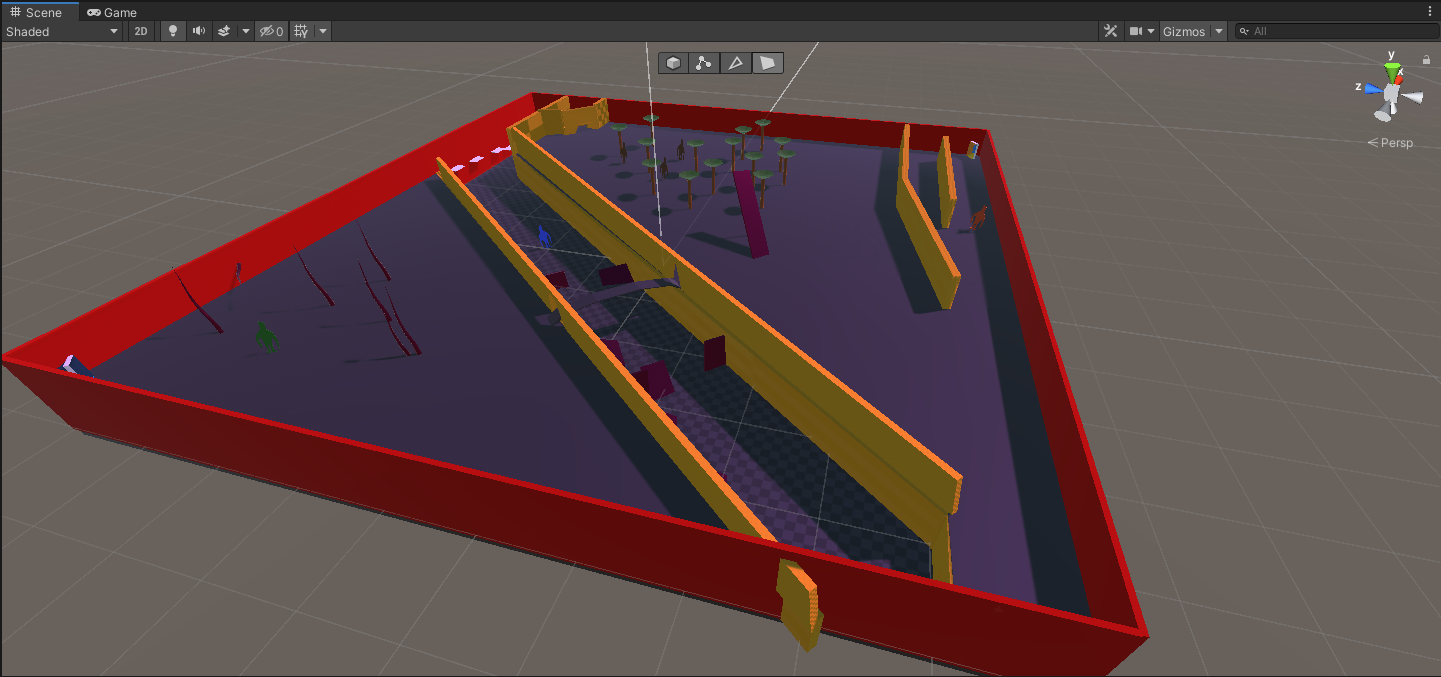
\includegraphics[scale=0.33]{Figures/level.png}
\caption{Individual First Level}
\end{figure}


\subsection{Sprint 2: Initial Development}

\begin{minted}[
frame=lines,
framesep=2mm,
baselinestretch=1.2,
bgcolor=gray!10,
fontsize=\footnotesize,
breaklines, 
linenos,
]{csharp}
/*OnFloor() checks if player is on ground
     * part of ground detection system
     */
    private bool OnFloor() 
    {
        //array of raycasts? to check if touching "floor"
        Collider[] hitColliders = Physics.OverlapBox(transform.position, transform.localScale / 3f, Quaternion.Euler(0, 0, 0), floorMask);
        bool check = false;
        //cycle through array >> if none true then not on floor, if just one, on floor
        for (int i = 0; i < hitColliders.Length; i++)
        {
            if (hitColliders[i]) 
            {
                check = true;
            }
        }
        return check;
    }
\end{minted}

\begin{figure}[H]
\centering
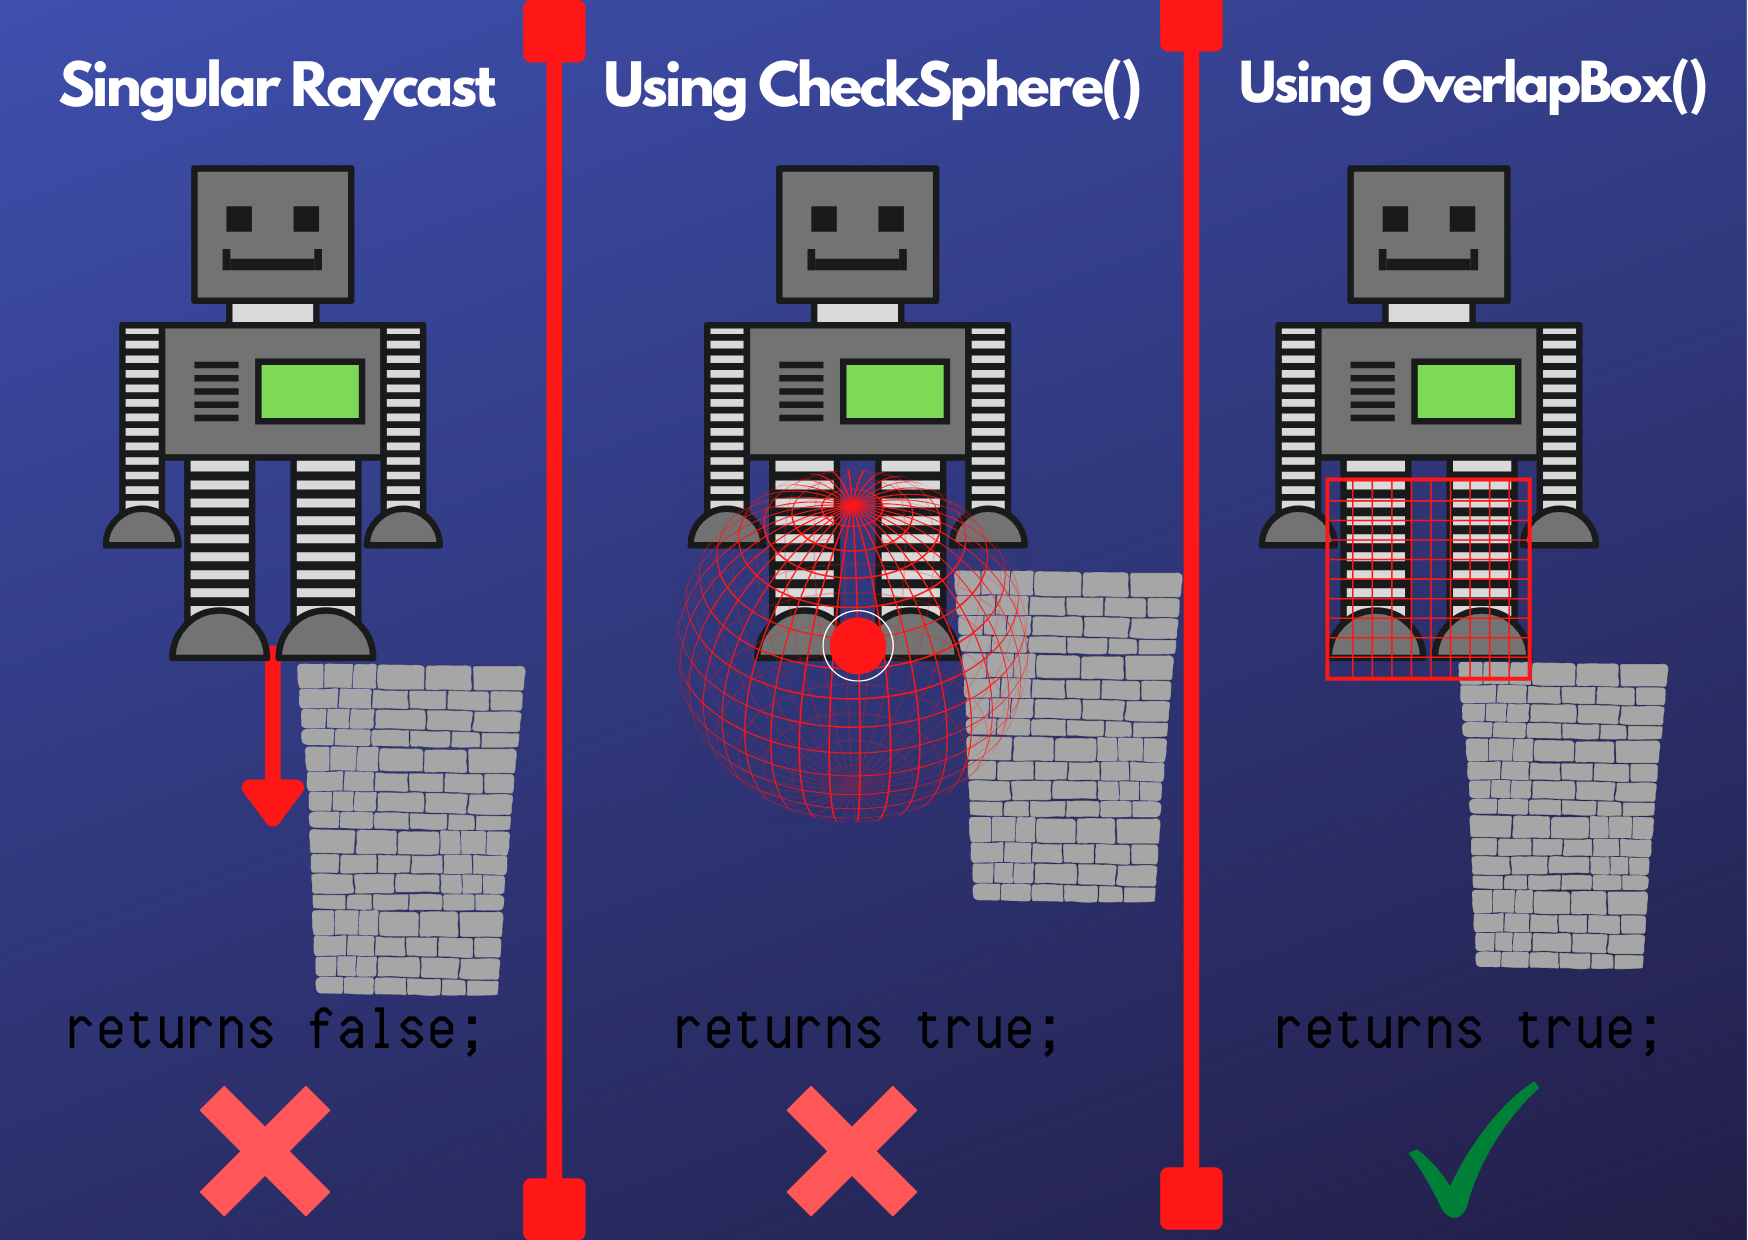
\includegraphics[scale=0.8]{Figures/floor.png}
\caption{Floor Detection Visualisation (Own Creation)}
\label{floor}
\end{figure}

\begin{figure}[H]
\centering
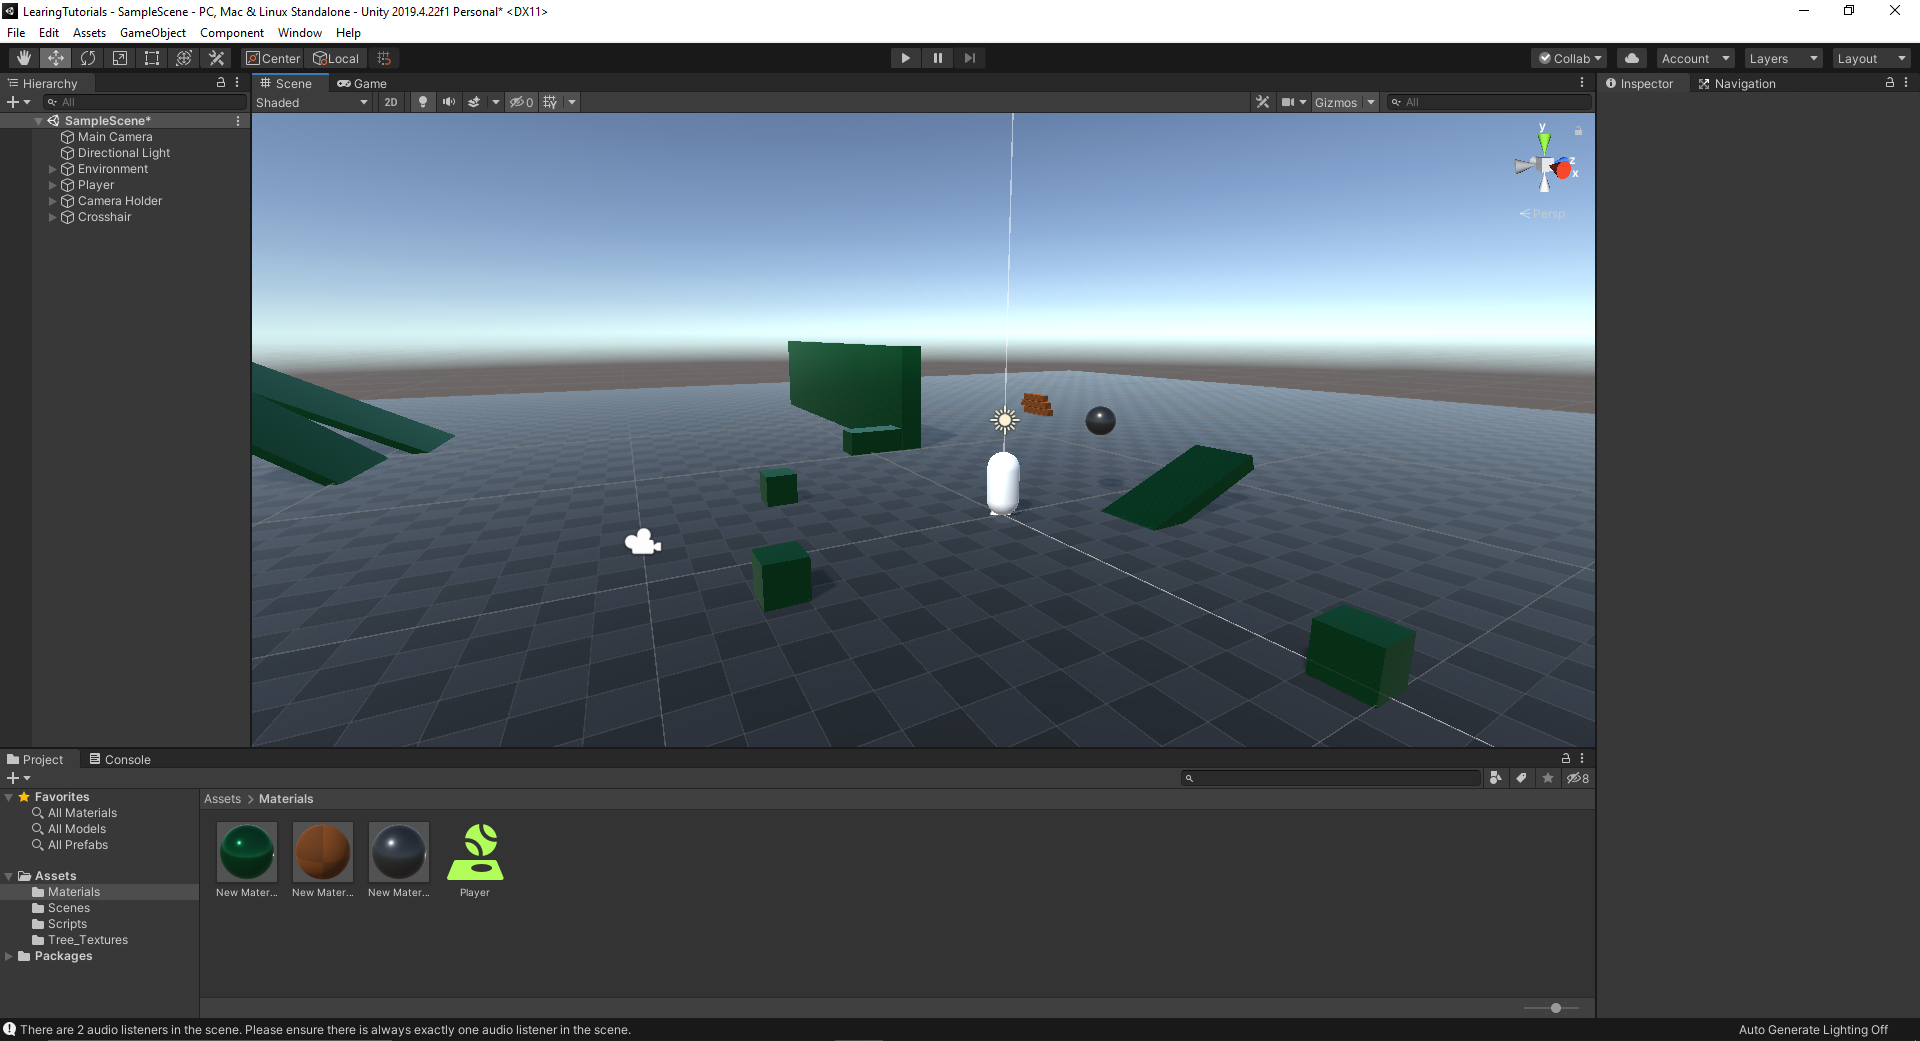
\includegraphics[scale=0.33]{Figures/testold.png}
\caption{Test Scene for Initial Player Movement}
\end{figure}




\subsection{Sprint 3: Full Scale Development}


\begin{figure}[H]
\centering
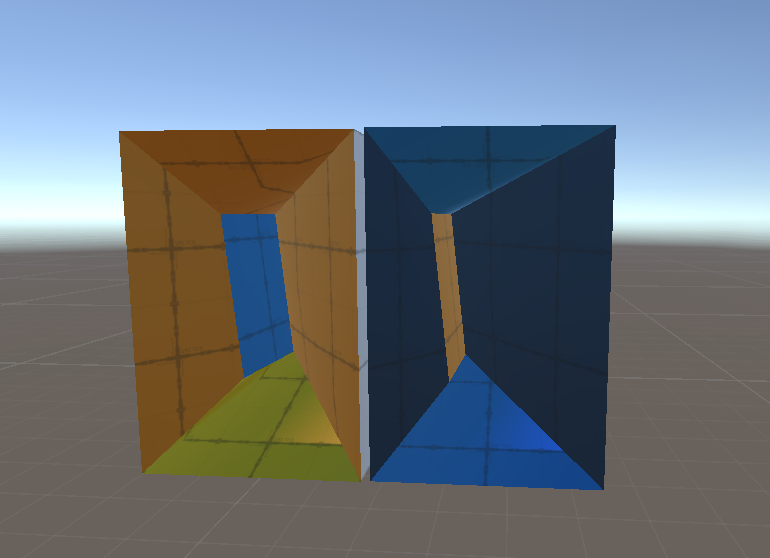
\includegraphics[scale=0.33]{Figures/portalconcept.png}
\caption{Original Portal Concept}
\end{figure}

\begin{figure}[H]
\centering
\begin{subfigure}{0.5\textwidth}
  \centering
  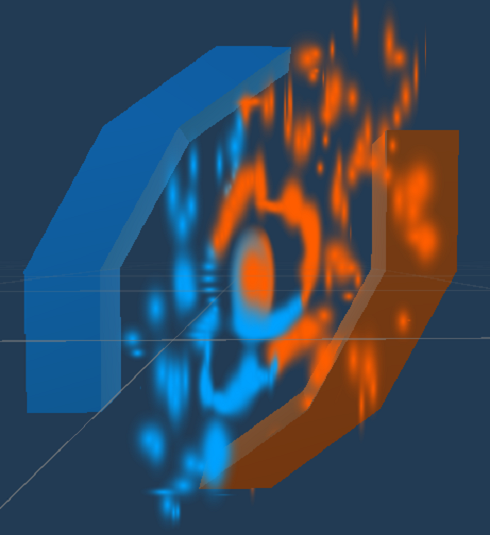
\includegraphics[width=1\linewidth]{Figures/finporta.png}
  \caption{Main Portal Asset}
\end{subfigure}%
\begin{subfigure}{0.5\textwidth}
  \centering
  
\includegraphics[width=1\linewidth]{Figures/finportb.png}
  \caption{Tutorial Specific Re-colouration}
\end{subfigure}
\caption{Finalised Portal Assest}
\end{figure}

%Full Level
\begin{figure}[H]
\centering
\begin{subfigure}{0.5\textwidth}
  \centering
  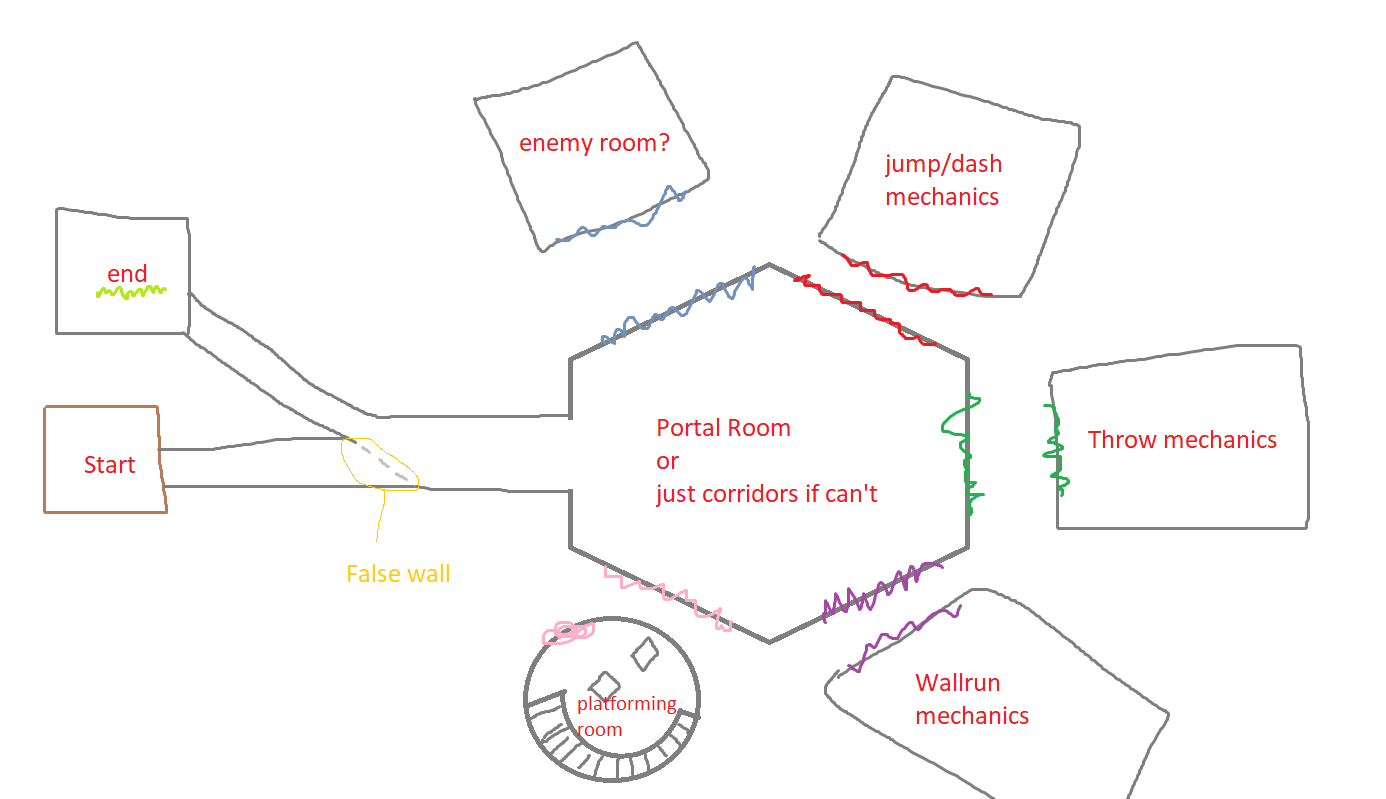
\includegraphics[width=1\linewidth]{Figures/fullplan.png}
  \caption{Provisional Plan}
\end{subfigure}%
\begin{subfigure}{0.5\textwidth}
  \centering
  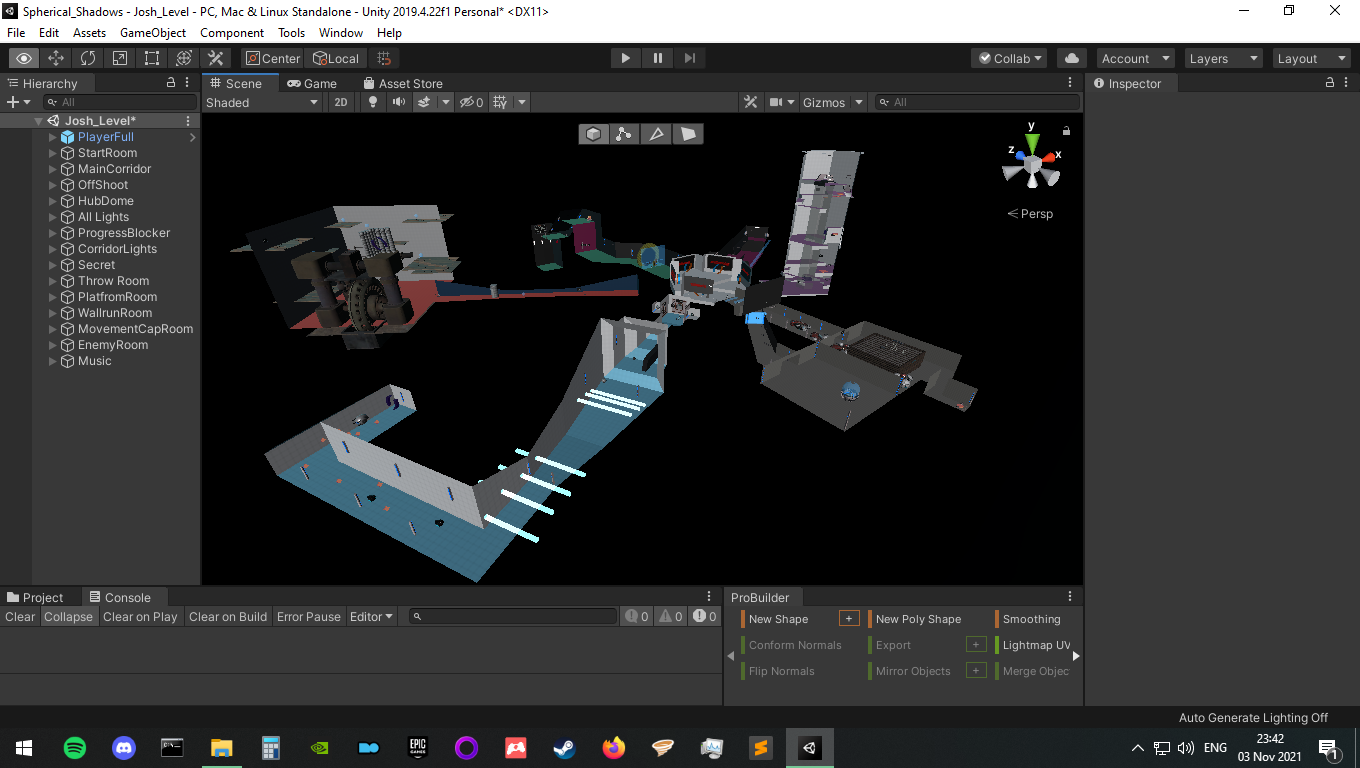
\includegraphics[width=1\linewidth]{Figures/full.png}
  \caption{Screenshot in Unity Editor}
\end{subfigure}
\caption{Layout of Full Level (Tutorial)}
\end{figure}


%Hub
\begin{figure}[H]
\centering
\begin{subfigure}{0.5\textwidth}
  \centering
  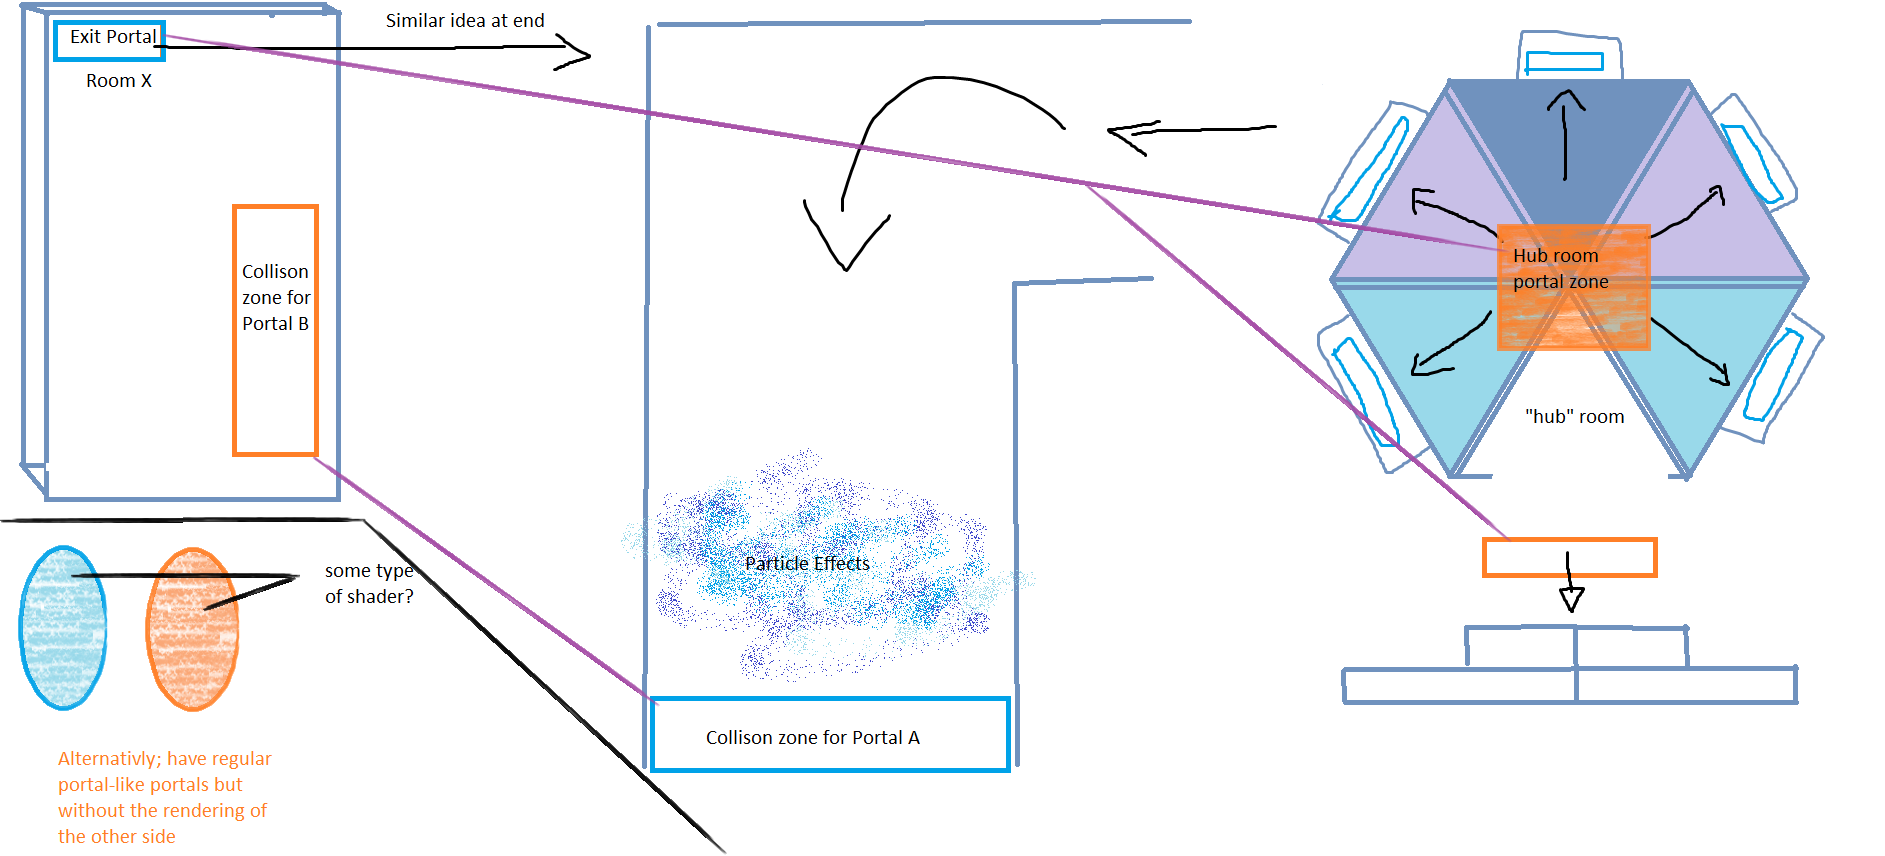
\includegraphics[width=1\linewidth]{Figures/hubplan.png}
  \caption{Provisional Plan}
\end{subfigure}%
\begin{subfigure}{0.5\textwidth}
  \centering
  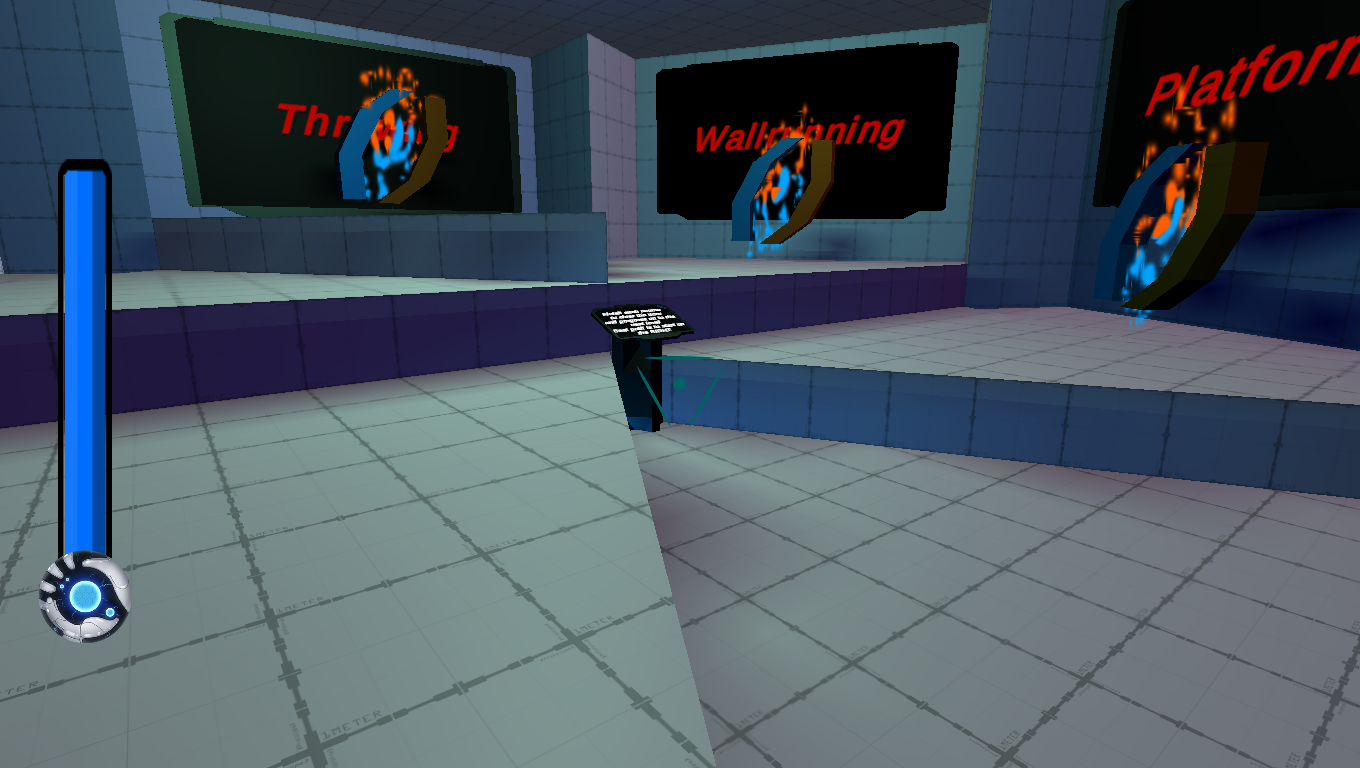
\includegraphics[width=1\linewidth]{Figures/hub.png}
  \caption{Screenshot in Artefact}
\end{subfigure}
\caption{Layout of Hub Room}
\end{figure}


%Platform
\begin{figure}[H]
\centering
\begin{subfigure}{0.5\textwidth}
  \centering
  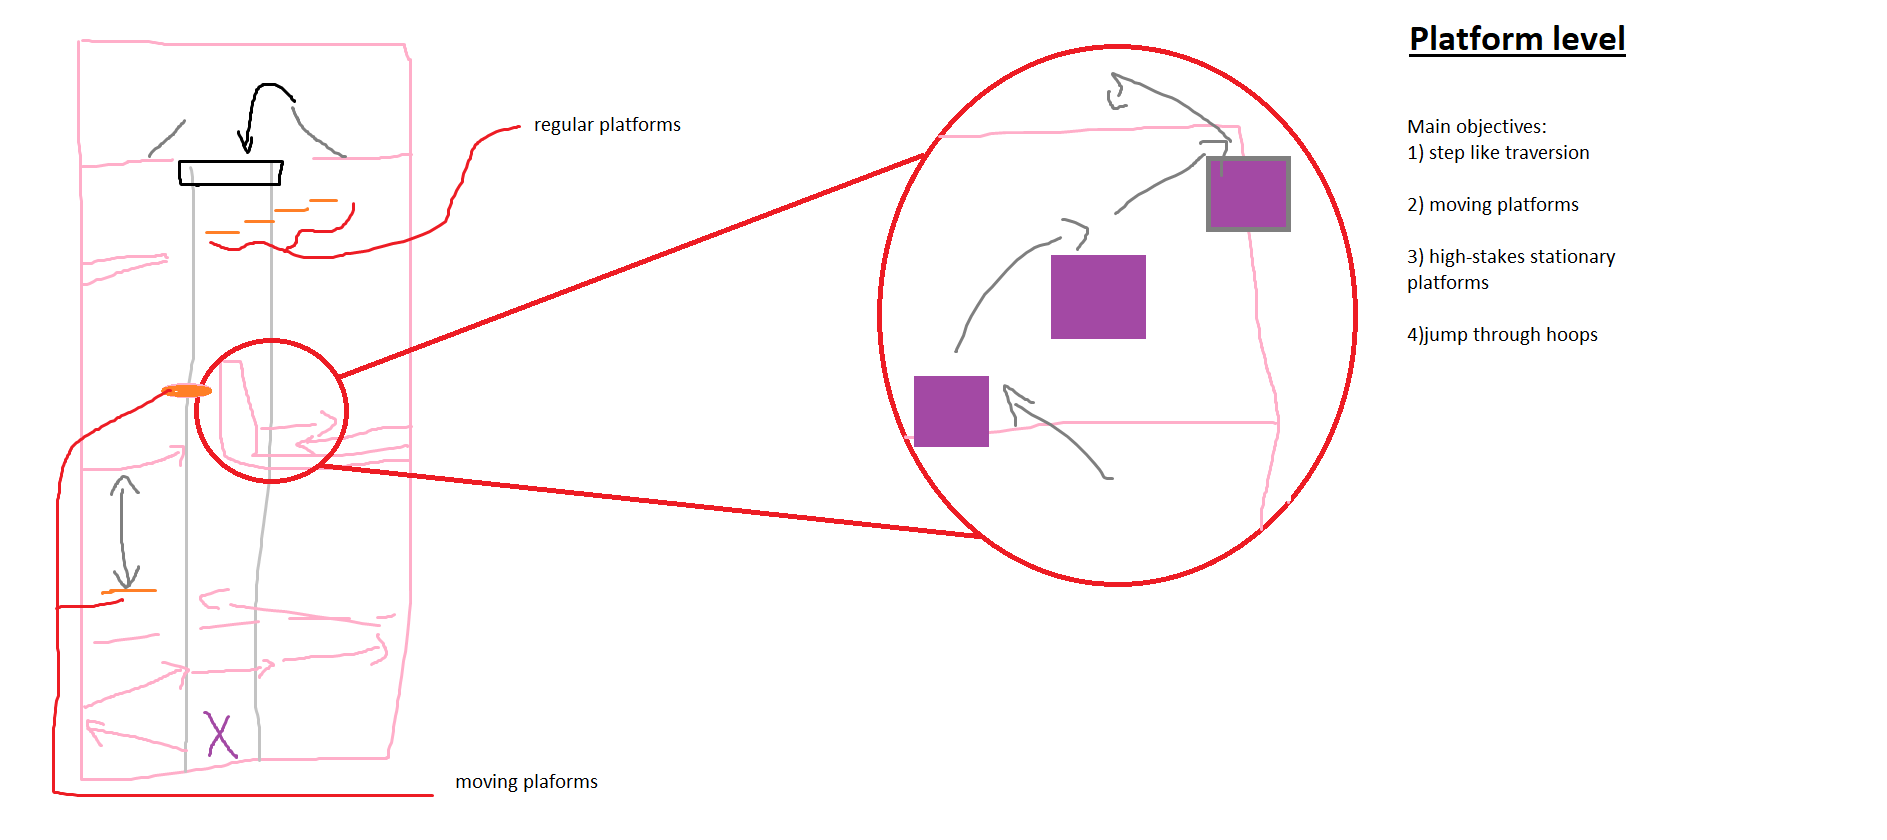
\includegraphics[width=1\linewidth]{Figures/platformplan.png}
  \caption{Provisional Plan}
\end{subfigure}%
\begin{subfigure}{0.5\textwidth}
  \centering
  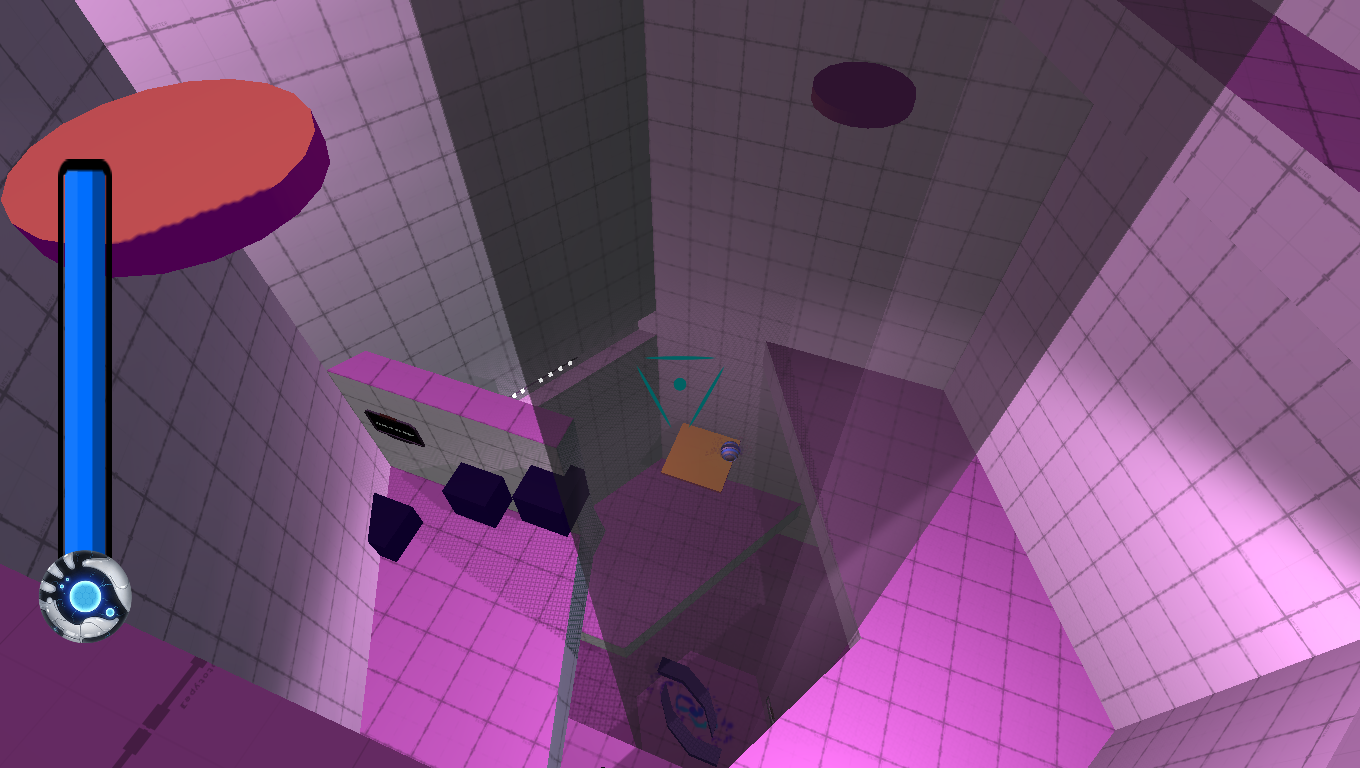
\includegraphics[width=1\linewidth]{Figures/platform.png}
  \caption{Screenshot in Artefact}
\end{subfigure}
\caption{Layout of Platforming Tutorial}
\end{figure}

%WallRun
\begin{figure}[H]
\centering
\begin{subfigure}{0.5\textwidth}
  \centering
  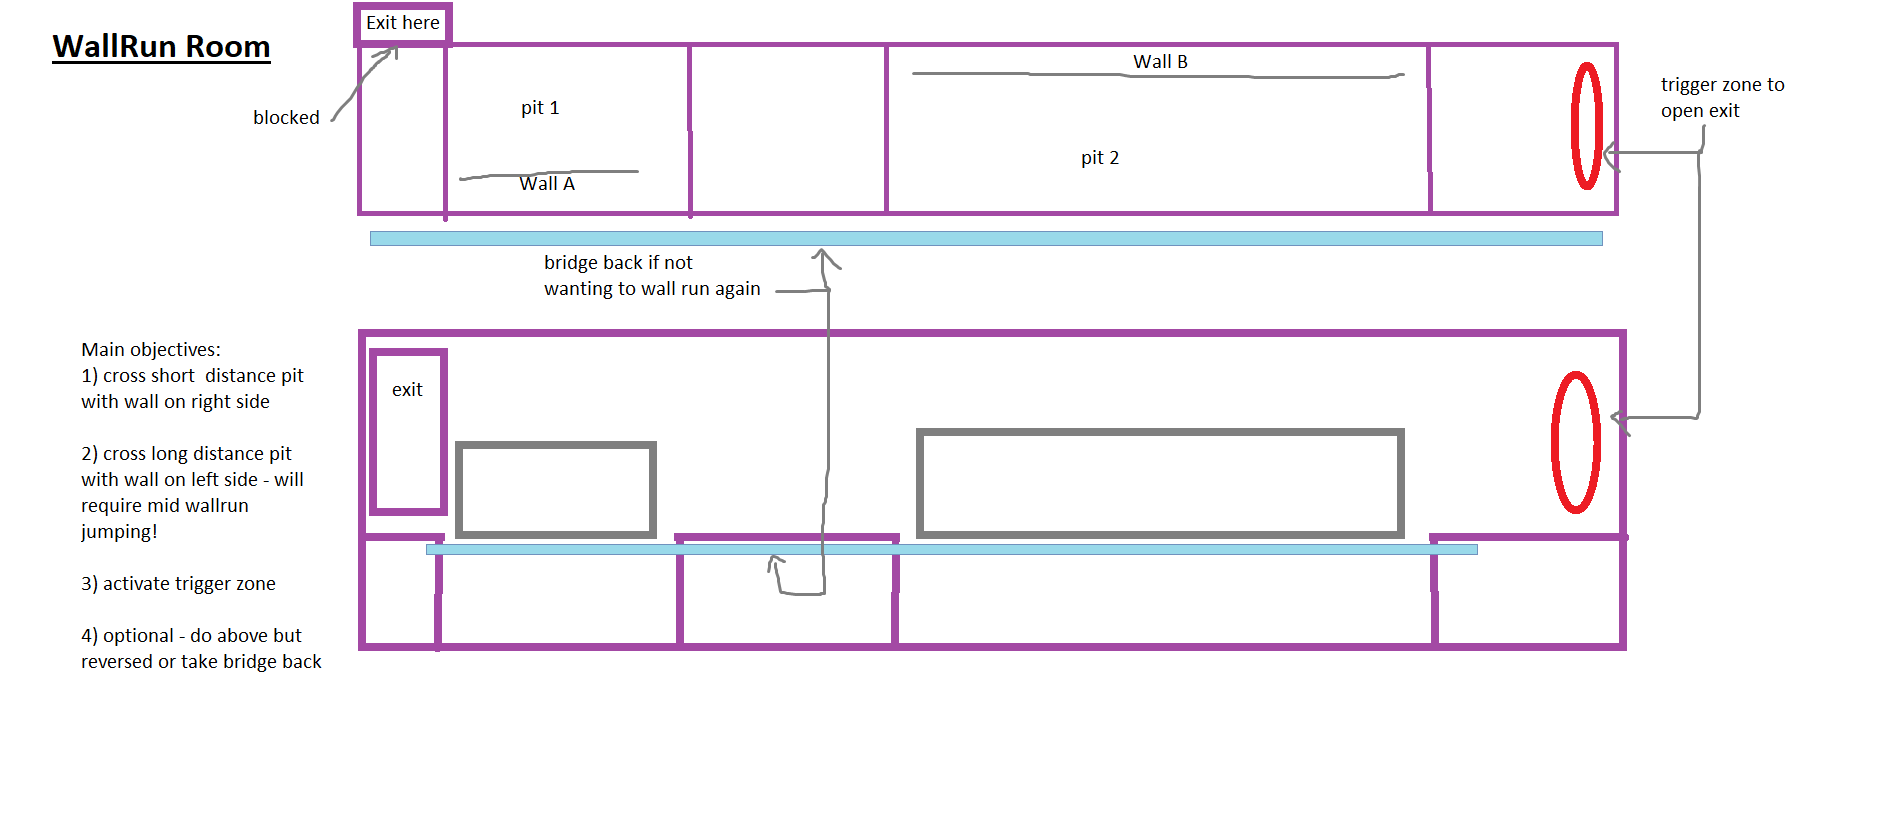
\includegraphics[width=1\linewidth]{Figures/wallplan.png}
  \caption{Provisional Plan}
\end{subfigure}%
\begin{subfigure}{0.5\textwidth}
  \centering
  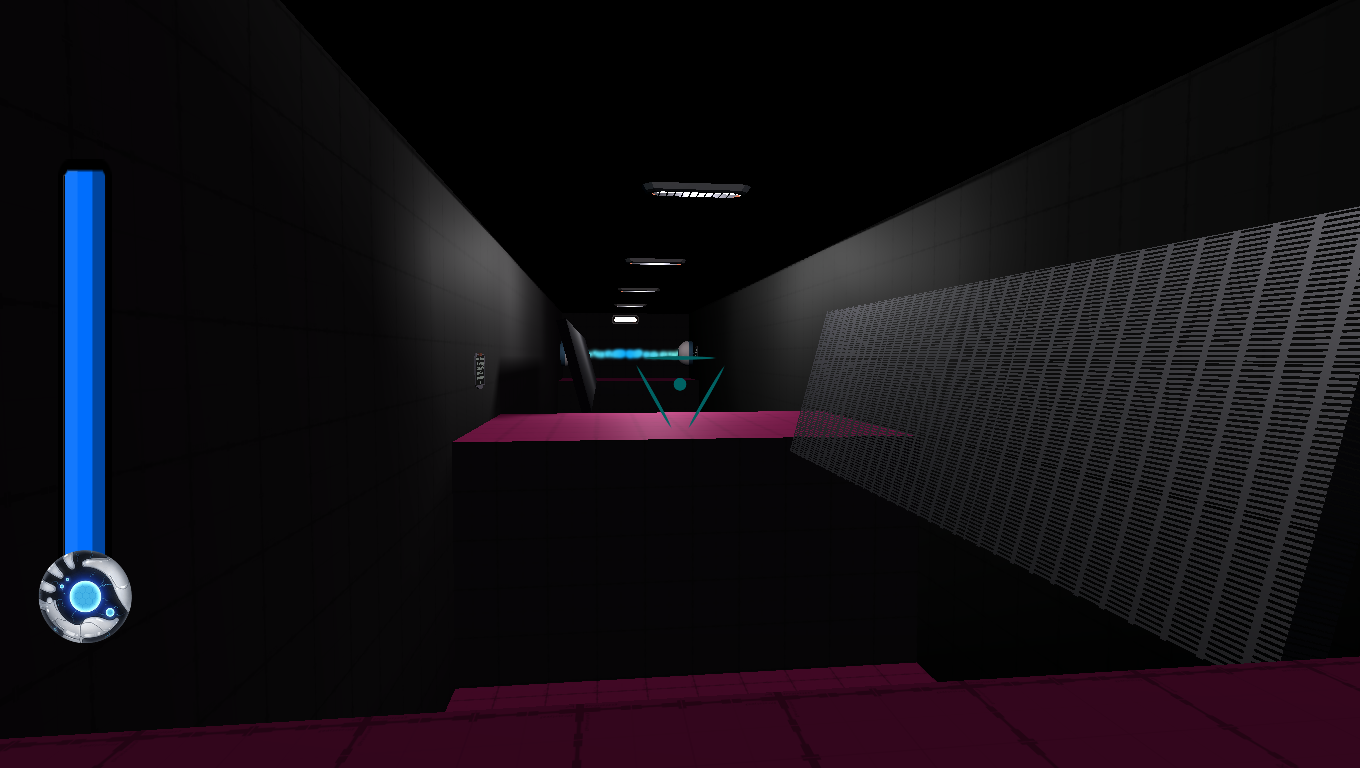
\includegraphics[width=1\linewidth]{Figures/wall.png}
  \caption{Screenshot in Artefact}
\end{subfigure}
\caption{Layout of Wall Running Tutorial}
\end{figure}

%Throw
\begin{figure}[H]
\centering
\begin{subfigure}{0.5\textwidth}
  \centering
  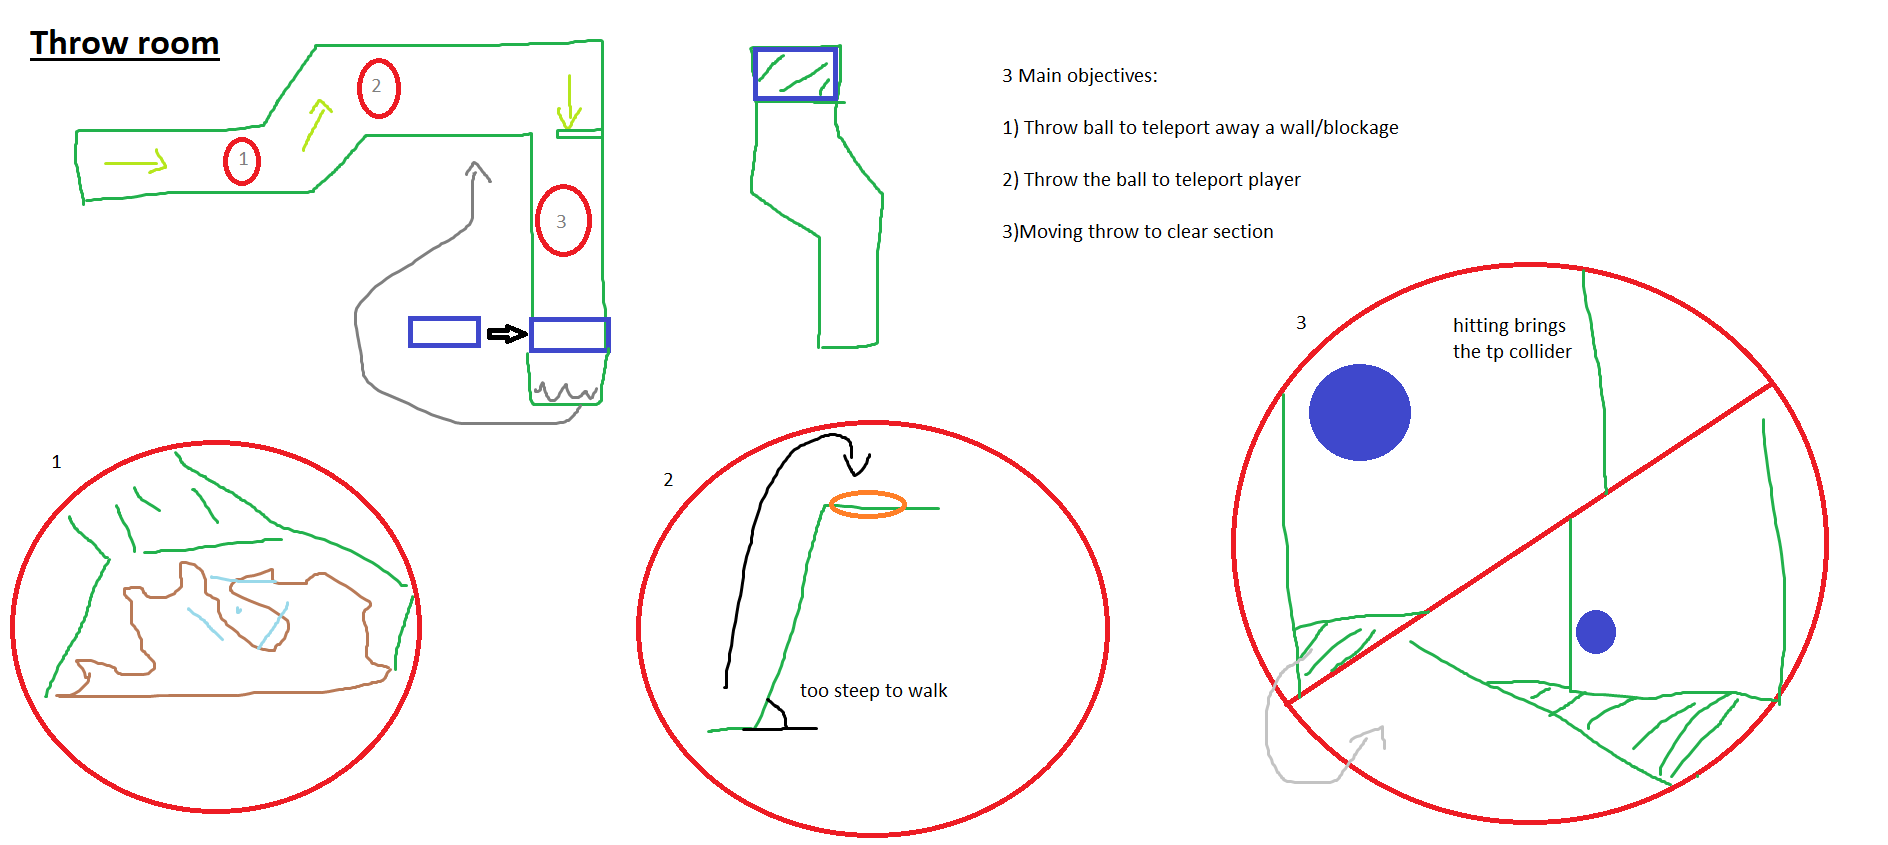
\includegraphics[width=1\linewidth]{Figures/throwplan.png}
  \caption{Provisional Plan}
\end{subfigure}%
\begin{subfigure}{0.5\textwidth}
  \centering
  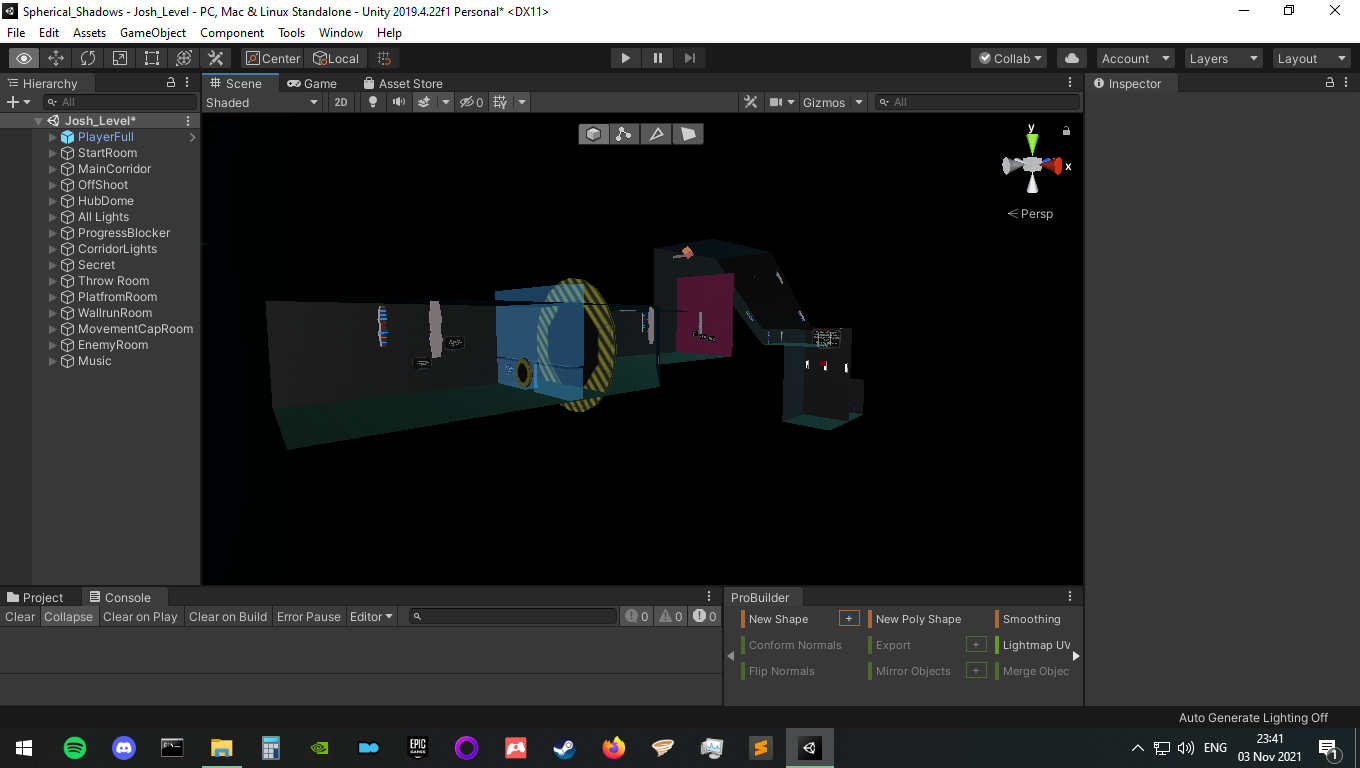
\includegraphics[width=1\linewidth]{Figures/throw.png}
  \caption{Screenshot in Unity Editor}
\end{subfigure}
\caption{Layout of Throw Tutorial}
\end{figure}


%Mcap
\begin{figure}[H]
\centering
\begin{subfigure}{0.5\textwidth}
  \centering
  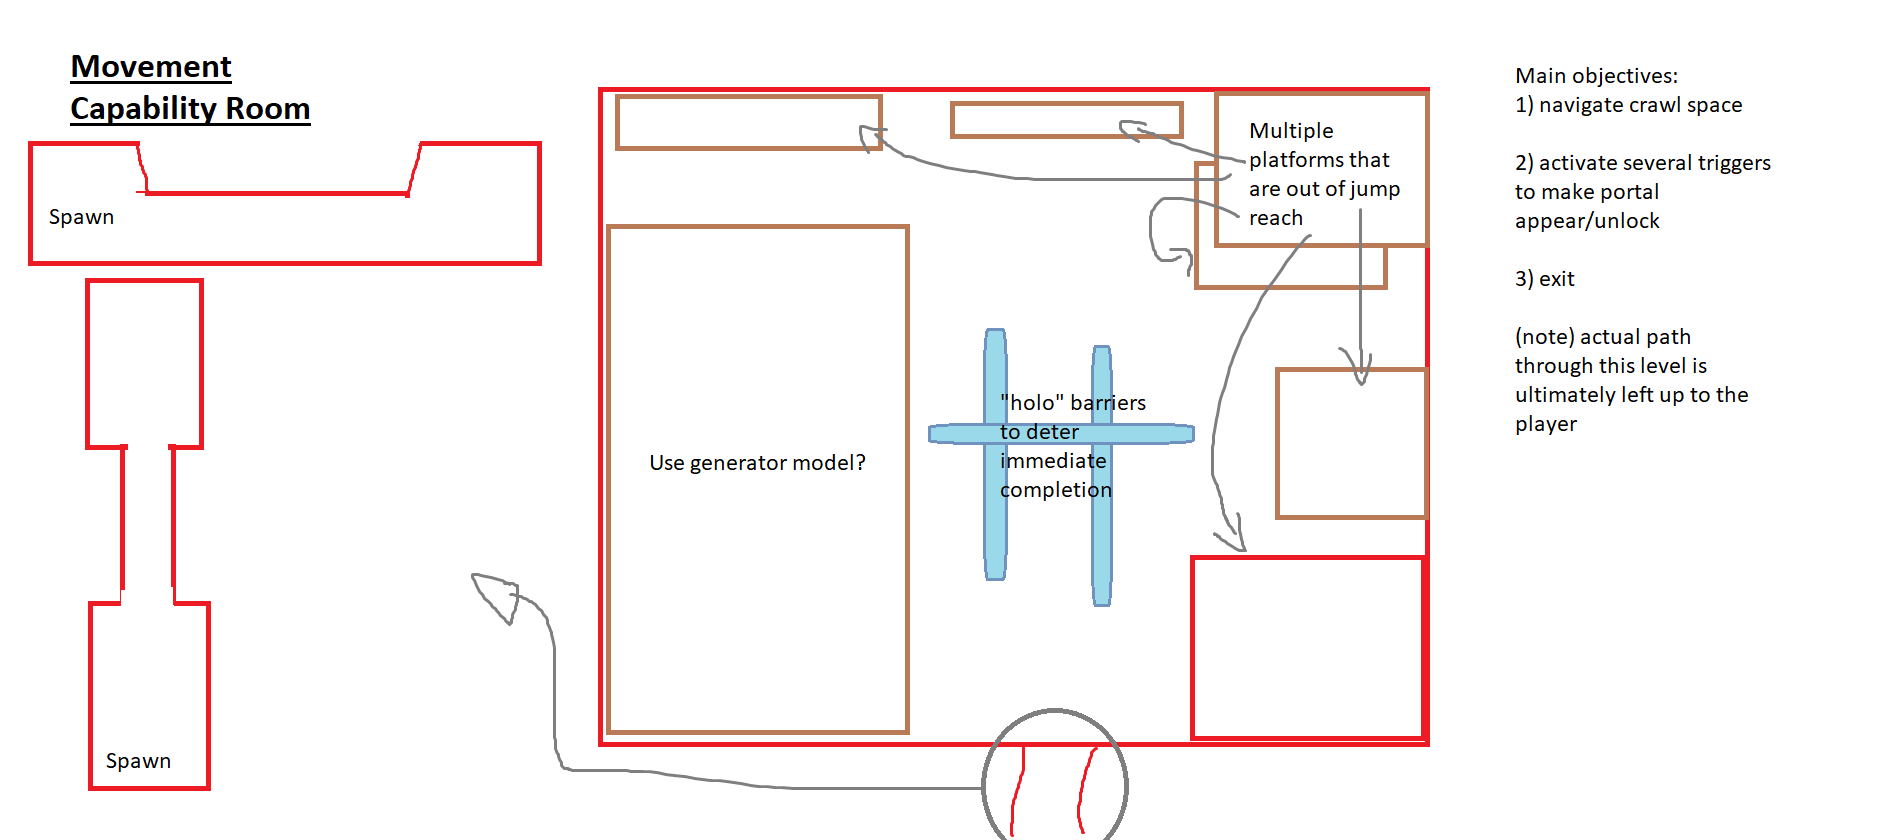
\includegraphics[width=1\linewidth]{Figures/mcapplan.png}
  \caption{Provisional Plan}
\end{subfigure}%
\begin{subfigure}{0.5\textwidth}
  \centering
  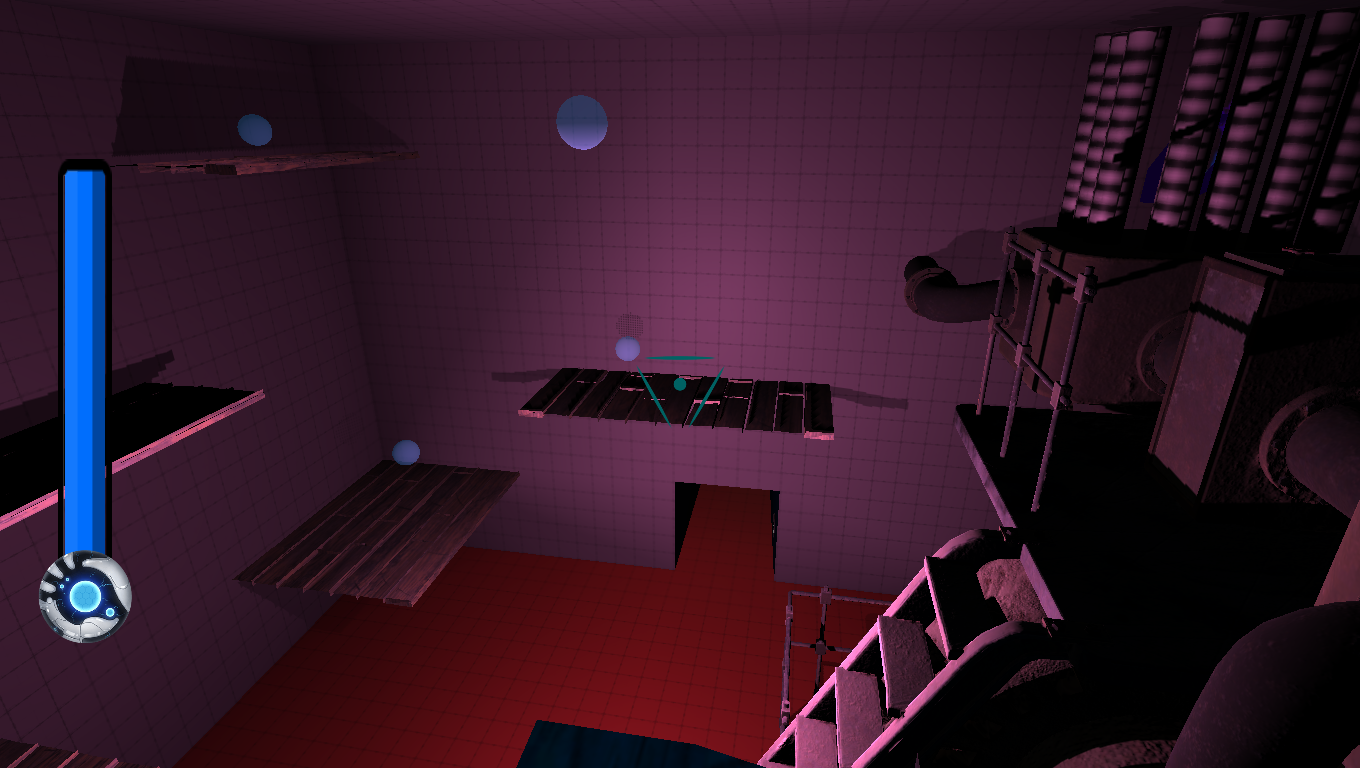
\includegraphics[width=1\linewidth]{Figures/mcap.png}
  \caption{Screenshot in Artefact}
\end{subfigure}
\caption{Layout of Movement Tutorial}
\end{figure}

%Enemy
\begin{figure}[H]
\centering
\begin{subfigure}{0.5\textwidth}
  \centering
  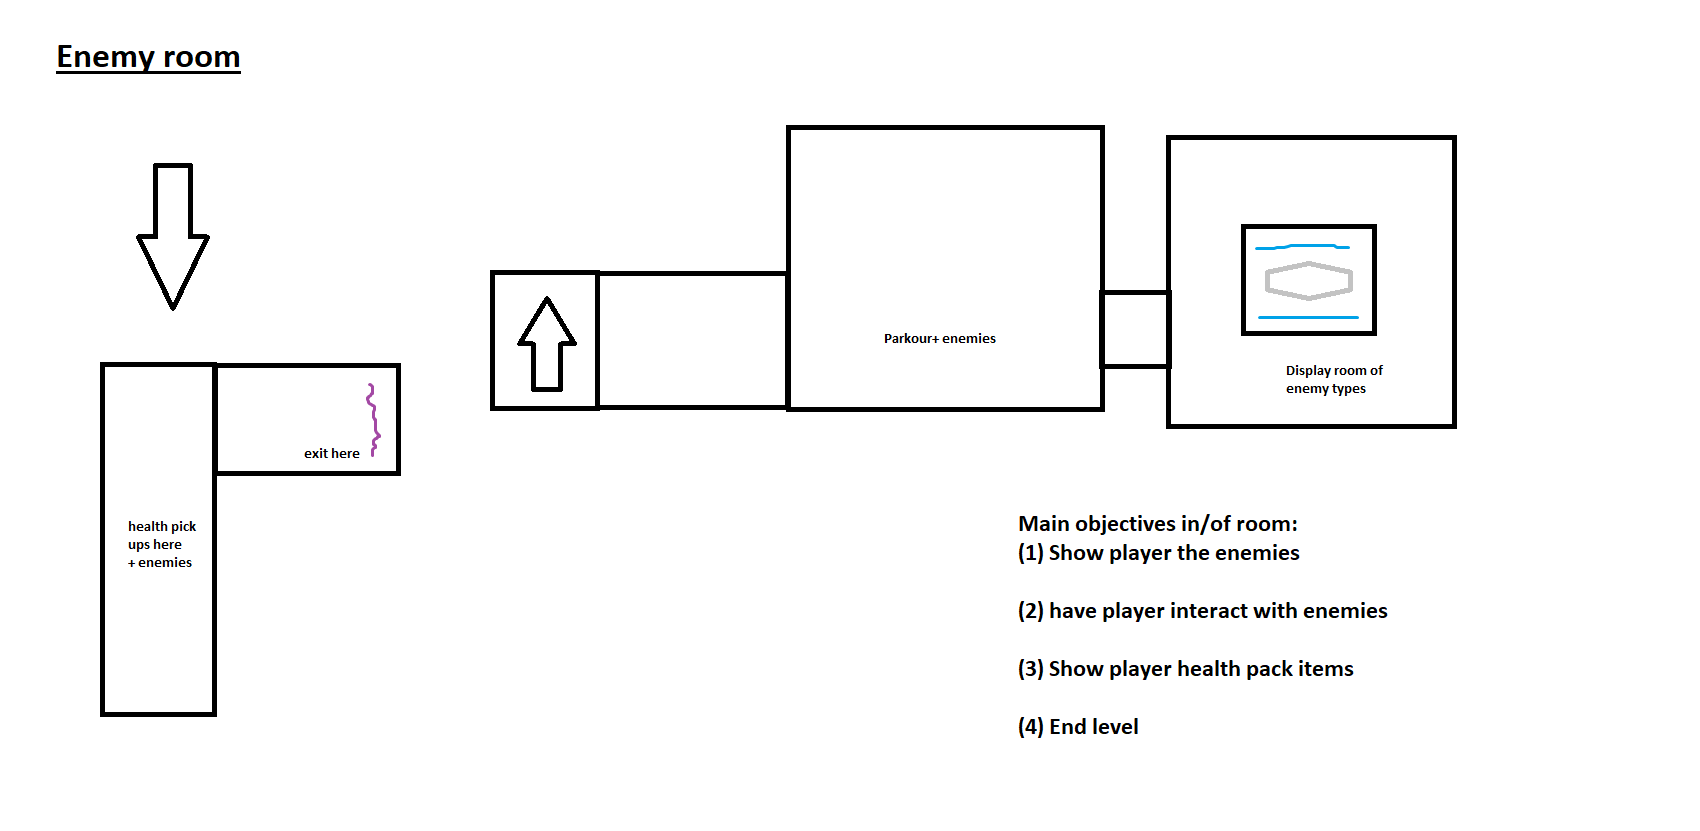
\includegraphics[width=1\linewidth]{Figures/enemyplan.png}
  \caption{Provisional Plan}
\end{subfigure}%
\begin{subfigure}{0.5\textwidth}
  \centering
  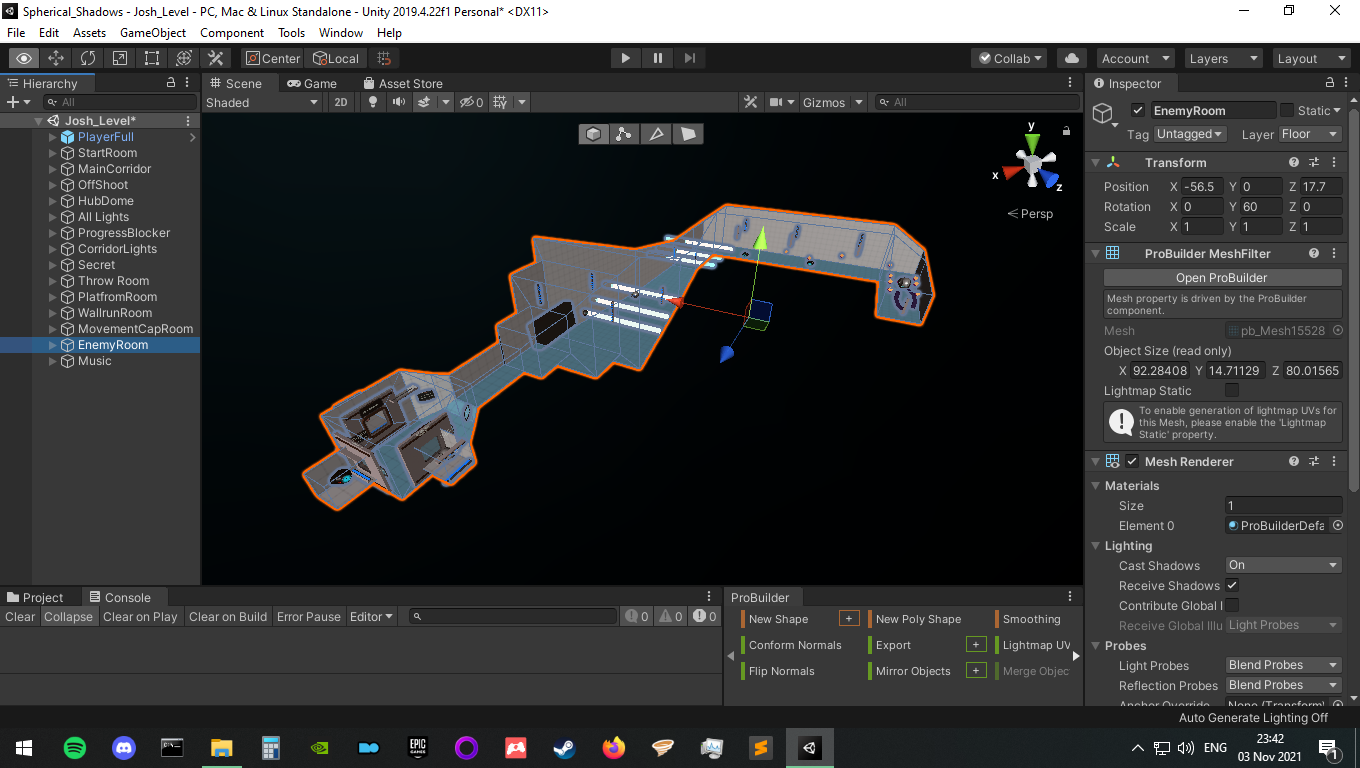
\includegraphics[width=1\linewidth]{Figures/enemy.png}
  \caption{Screenshot in Unity Editor}
\end{subfigure}
\caption{Layout of Enemy Tutorial}
\end{figure}


\begin{figure}[H]
\centering
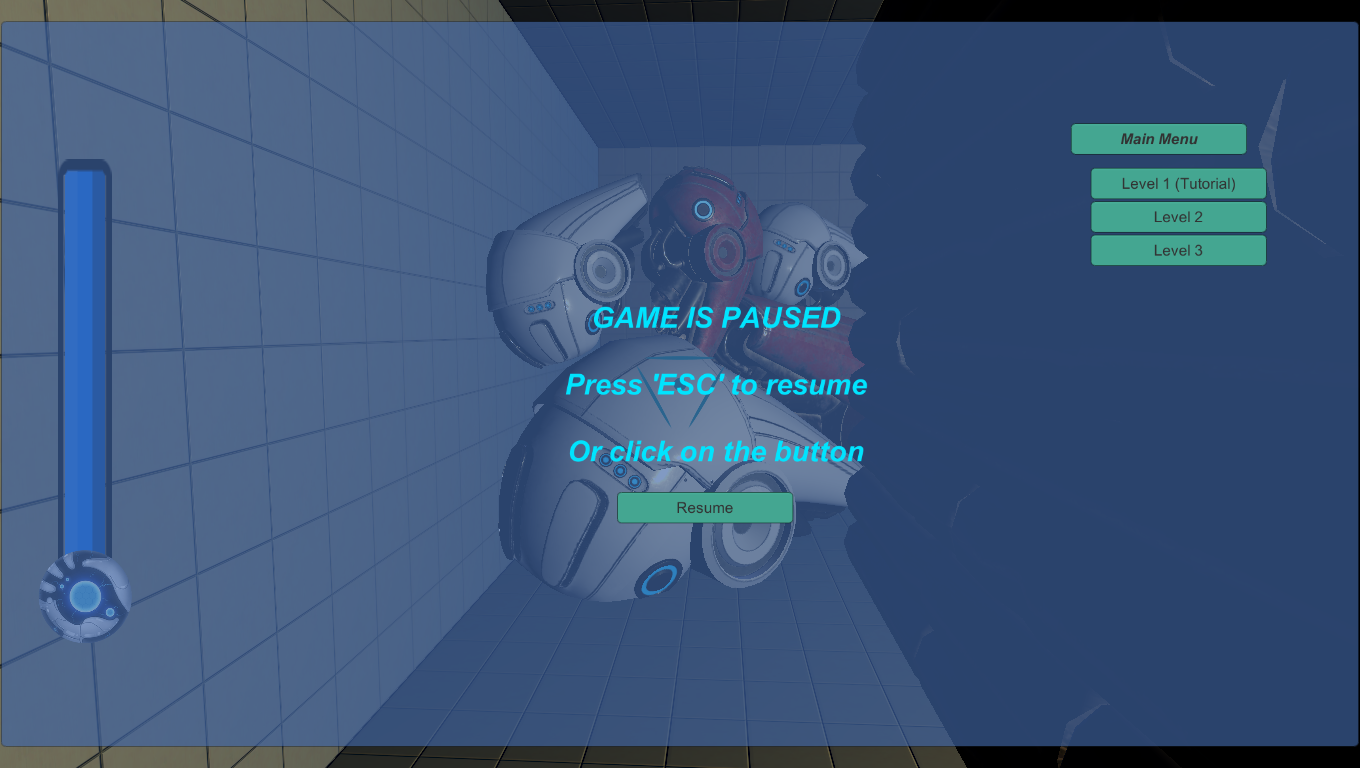
\includegraphics[scale=0.45]{Figures/pause.png}
\caption{Pause Menu}
\end{figure}

\subsection{Sprint 4: Build and Publish}



\begin{figure}[H]
\centering
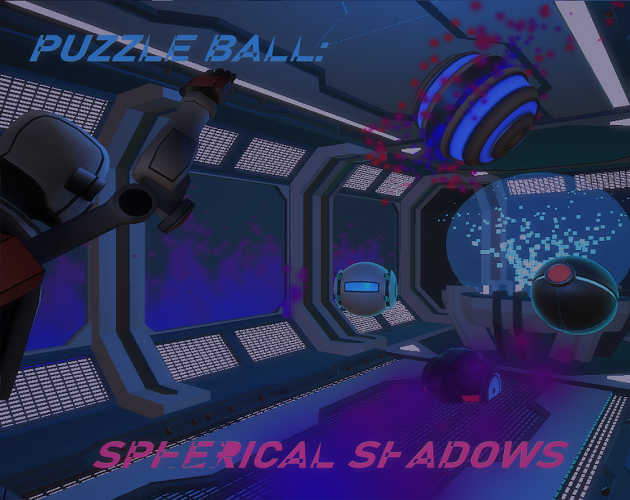
\includegraphics[scale=0.6]{Figures/thumb.png}
\caption{The Icon Used for Publication}
\end{figure}

\section{Description of the Development of the Article}
%Comprehensive report on the way in which each phase of the life cycle was applied in the development of this artefact.

\subsection{Sprint 1: Research Proposal}

\subsection{Sprint 2: Project Planning}

\subsection{Sprint 3: Sampling and Literature Collection}

\subsection{Sprint 4: Write Article}

\subsection{Sprint 5: Finalise Article}




\section{Conclusion}